% 61-17(61쪽) — 이차함수 f 의 도함수 y=f'(x)(직선)와 삼차함수 g 의 도함수 y=g'(x)(아래로 볼록한 포물선). 스캔 화질이 낮아 TikZ 로 다시 그림.
% 원문에 있는 것만: x축 위 문자 a b c d e · 라벨 O, x, y, y=f'(x), y=g'(x) · 안내 파선(b 는 축에서 아래로 두 그래프의 교점까지, e 는 축에서 위로 교점까지).
% 원문의 뜻: a · d 는 포물선의 x절편, c 는 직선의 x절편, b · e 는 두 그래프의 교점의 x좌표. 순서 a<b<c<O<d<e 를 그대로 지킨다.
% 포물선 y=0.30(x+4.2)(x-1.9), 직선 y=0.51(x+1.659) 로 두면 교점이 정확히 x=-3.6(b) · x=3.0(e) 이 되어 원문 배치와 같다. 눈금은 원문에 없으므로 넣지 않는다.
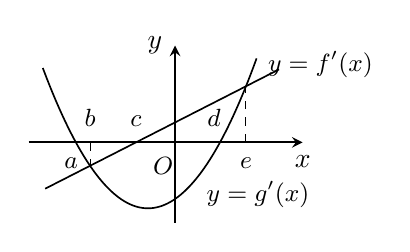
\begin{tikzpicture}[x=0.30cm, y=0.30cm, line width=0.5pt]
  \draw[->, >=stealth, line width=0.7pt] (-6.2,0) -- (5.4,0) node[below=1pt] {$x$};
  \draw[->, >=stealth, line width=0.7pt] (0,-3.4) -- (0,4.1) node[left=1pt] {$y$};
  \node[below=2pt, font=\small] at (-0.5,0) {$\pt{O}$};
  % 안내 파선(원문)
  \draw[dashed, line width=0.35pt] (-3.6,0) -- (-3.6,-0.99);
  \draw[dashed, line width=0.35pt] (3,0) -- (3,2.38);
  % 그래프
  \draw[line width=0.6pt, domain=-5.6:3.45, samples=80, smooth] plot (\x, {0.30*(\x+4.2)*(\x-1.9)});
  \draw[line width=0.6pt] (-5.5,-1.96) -- (4.4,3.09);
  % 문자(원문 자리 그대로: b · c · d 는 축 위, a · e 는 축 아래)
  \node[below=2pt, font=\small] at (-4.4,0) {$a$};
  \node[above=2pt, font=\small] at (-3.6,0) {$b$};
  \node[above=2pt, font=\small] at (-1.66,0) {$c$};
  \node[above=2pt, font=\small] at (1.65,0) {$d$};
  \node[below=2pt, font=\small] at (3,0) {$e$};
  \node[right=1pt, font=\small] at (3.4,3.3) {$y=f'(x)$};
  \node[right=1pt, font=\small] at (0.8,-2.2) {$y=g'(x)$};
\end{tikzpicture}
